\documentclass{article}

\usepackage[utf8]{inputenc}
\usepackage{titlesec}
\usepackage{easylist}
\usepackage{hanging}
\usepackage{hyperref}
\usepackage[a4paper,top=2.0cm,bottom=2.0cm,left=2.0cm,right=2.0cm]{geometry}
\usepackage{blindtext}
\usepackage{tipa}
\usepackage{epigraph}
\usepackage{enumerate}
\usepackage{longtable}
\usepackage{setspace}
\usepackage{verbatim}
\usepackage[T1]{fontenc}
\usepackage{graphicx}
\usepackage[italian]{babel}
\usepackage{amsmath}
\usepackage{pbox}
\usepackage{fancyhdr}
\usepackage{cancel}
\usepackage{tabularx}
\usepackage{booktabs}
\usepackage{multirow}
\usepackage{longtable}
\usepackage{tikz}
\usepackage{tikz-qtree}
\usepackage{subfig}
\usepackage{xcolor}
\usepackage{amssymb}
\usepackage{mathrsfs}
\usepackage{textcomp}

\usepackage{listings}
\usepackage{color}

\definecolor{mygreen}{rgb}{0,0.6,0}
\definecolor{mygray}{rgb}{0.5,0.5,0.5}
\definecolor{mymauve}{rgb}{0.58,0,0.82}

\lstset{ 
  backgroundcolor=\color{white},   % choose the background color; you must add \usepackage{color} or \usepackage{xcolor}; should come as last argument
  basicstyle=\footnotesize,        % the size of the fonts that are used for the code
  breakatwhitespace=false,         % sets if automatic breaks should only happen at whitespace
  breaklines=true,                 % sets automatic line breaking
  captionpos=b,                    % sets the caption-position to bottom
  commentstyle=\color{mygreen},    % comment style
  deletekeywords={...},            % if you want to delete keywords from the given language
  escapeinside={\%*}{*)},          % if you want to add LaTeX within your code
  extendedchars=true,              % lets you use non-ASCII characters; for 8-bits encodings only, does not work with UTF-8
  firstnumber=1000,                % start line enumeration with line 1000
  frame=single,	                   % adds a frame around the code
  keepspaces=true,                 % keeps spaces in text, useful for keeping indentation of code (possibly needs columns=flexible)
  keywordstyle=\color{blue},       % keyword style
  language=Octave,                 % the language of the code
  morekeywords={*,...},            % if you want to add more keywords to the set
  numbers=left,                    % where to put the line-numbers; possible values are (none, left, right)
  numbersep=5pt,                   % how far the line-numbers are from the code
  numberstyle=\tiny\color{mygray}, % the style that is used for the line-numbers
  rulecolor=\color{black},         % if not set, the frame-color may be changed on line-breaks within not-black text (e.g. comments (green here))
  showspaces=false,                % show spaces everywhere adding particular underscores; it overrides 'showstringspaces'
  showstringspaces=false,          % underline spaces within strings only
  showtabs=false,                  % show tabs within strings adding particular underscores
  stepnumber=2,                    % the step between two line-numbers. If it's 1, each line will be numbered
  stringstyle=\color{mymauve},     % string literal style
  tabsize=2,	                   % sets default tabsize to 2 spaces
  title=\lstname                   % show the filename of files included with \lstinputlisting; also try caption instead of title
}

\linespread{1.5} % l'interlinea

\frenchspacing

\newcommand{\abs}[1]{\lvert#1\rvert}

\usepackage{floatflt,epsfig}

\usepackage{multicol}
\newcommand\yellowbigsqcup[1][\displaystyle]{%
  \fboxrule0pt
  \ifx#1\textstyle\fboxsep-0.6pt\else\fboxsep-1.25pt\fi
  \mathrel{\fcolorbox{white}{yellow}{$#1\bigsqcup$}}}

\title{Prontuario Fisica 1}
\author{Nicola Ferru}

\newtheorem{teo}{Teorema}
\begin{document}
\maketitle

\section{Vettori}
\label{sec:vect}

\subsection{Triangolo rettangolo: sin, cos e tan}
\label{sec:triangoretsincosetan}
\begin{eqnarray}
  \label{eq:sincostan}
  \cos \alpha = \frac{AB}{BC}\\
  \sin \alpha = \frac{AC}{BC}\\
  \tan \alpha = \frac{AC}{AB}
\end{eqnarray}

\subsection{Teorema di Carno sui triangoli}
\label{sec:carnoetriang}

\begin{eqnarray}
  \label{eq:teoremadicarnot}
  a^2=b^2+c^2-2bc\cdot \cos\alpha\\
  b^2=a^2+c^2-2ac \cdot \cos \beta\\
  c^2=b^2+a^2-2ba\cdot \cos \gamma
\end{eqnarray}

\subsection{teorema dei seni}
\label{teorseni}

\begin{eqnarray}
  \label{eq:sin}
  \frac{a}{\sin \alpha} = \frac{b}{\sin \beta} = \frac{c}{\sin \gamma}
\end{eqnarray}

\subsection{Algebra vettoriale}
\label{sec:algvett}

\begin{eqnarray}
  \label{eq:algvet}
  \text{Somma di vettori: } a+b=c
\end{eqnarray}

\subsubsection{Scomposizione di vettore}
\label{sec:scomposizione}

\begin{eqnarray}
  \label{eq:scompvetto}
  v_x=v\cos \alpha\\
  v_y=v\sin \alpha{}\\
  v=\sqrt{(v_x^2+v_y^2)}
\end{eqnarray}

\subsubsection{prodotti tra due vettori}
\label{sec:prodtraduevett}

\begin{eqnarray}
  \label{eq:prodtraduevett}
  \text{prodotto scalare: }a\cdot b=ab\cos \alpha{}\\
  \text{prodotto vettoriale:}a \times b=c
\end{eqnarray}

\section{Velocità}
\label{sec:velocità}

\subsection{velocità media}
\label{sec:velmedia}


\begin{eqnarray}
  \label{eq:velmedia}
  \bar{V} = \frac{\Delta x_{totale}}{\Delta t_{totale}}=\frac{x_2-x_1}{t_2-t_1}
\end{eqnarray}

\subsection{km/h a m/s}
\label{sec:km/hm/s}

\subsection{Accelerazione}
\label{sec:accelerarzione}

\begin{eqnarray}
  \label{eq:acc}
  \bar{a}=\frac{v_2-v_1}{t_2-t_1}=\frac{\Delta v}{\Delta t}\\
  v=v_0+at\\
  x=x_0+\bar{v} t
\end{eqnarray}

\subsection{Legge oraria}
\label{sec:leggeoraria}

\begin{eqnarray}
  \label{eq:leggeo}
  x=x_0+v_0t + \frac{1}{2} at^2\\
  x=vt+\frac{1}{2} at^2
\end{eqnarray}


\section{Moti}
\label{sec:moti}
\subsection{Moto in caduta libera}
\label{sec:motocadutalibera}

\begin{eqnarray}
  \label{eq:cadutalibera}
  y=v_0t-\frac{1}{2}gt^2
\end{eqnarray}

\subsection{Moto orizzontale}
\label{sec:motooriz}

\begin{eqnarray}
  \label{eq:motooriz}
  x-x_0=v_{0x}t=v_0\cos\Theta_0t
\end{eqnarray}

\subsection{Moto verticale}
\label{sec:motovert}

\begin{eqnarray}
  \label{eq:motovert}
  y-y_0=v_{0y}t-\frac{1}{2}gt^2=v_0\sin \Theta_0t-\frac{1}{2}gt^2
\end{eqnarray}

\subsection{Equazione delle traiettoria}
\label{sec:eqtrai}

\begin{eqnarray}
  \label{eq:eqtrai}
  t=\frac{x-x_0}{v_0\cos\Theta_0}\\
  y-y_0=v_0\sin\Theta_0\left(\frac{x-x_0}{v_0\cos\Theta_0}\right)-\frac{1}{2}g\left(\frac{x-x_0}{v_0\cos\Theta_0}\right)^2& \text{se }
                                                                                                                            \begin{matrix}
                                                                                                                              x_0=0\\
                     y_0=0
                                                                                                                            \end{matrix}\\
  y=\not{v_0}\sin\Theta_0\frac{x}{\not{v_0}\cos\Theta_0}-\frac{1}{2}g\frac{x^2}{v^2_0\cos^2\Theta_0}\to y=\underbrace{\tan\Theta_0}_Ax-\underbrace{\frac{gx^2}{2v_0^2\cos^2\Theta{}_0}}_B\\
  y=Ax-Bx^2
\end{eqnarray}

\subsection{La Gittata}
\label{sec:gittata}

\begin{eqnarray}
  \label{eq:gittata}
  \begin{cases}
    x-x_0=R\\
    y_0=0;\text{ }y=0
  \end{cases}\\
  \begin{cases}
    R=(v_0\cos\Theta_0)t\to t =\frac{R}{v_0\cos\Theta{}_0}\\
    O=(v_0\sin\Theta{}_0)-\frac{1}{2}t^2\to \not{v_0}\sin\Theta_0\frac{R}{\not{v_0}\cos\Theta_0}-\frac{1}{2}g\frac{R^2}{(v_0\cos\Theta_0)^2}
  \end{cases}\\
  v_0^2\sin\Theta{}\cos\Theta{}_0R-\frac{1}{2}R^2=0 & R\left(v_0^2\sin\Theta{}_0\cot\Theta{}_0-\frac{1}{2}gR\right)=0
\end{eqnarray}
Nel caso in cui $R_1$ dovesse essere nullo $R_2$ si calcola nel seguente modo:
\begin{eqnarray}
  \label{eq:R1=0}
  R_1=0\\
  R_2=\frac{2v_0}{g} \sin\Theta{}_0\cos\Theta{}_0=\underbrace{\frac{v_0^2}{g}\sin(2\Theta{}_0)}_{
  \begin{matrix}
    MAX\to \sin()=1\\
    2\Theta{}=90^o\to \Theta{}_0=45^o
  \end{matrix}
  }
\end{eqnarray}
\subsection{Il moto dei proiettili}
\label{sec:proiettili}

\begin{eqnarray}
  \label{eq:proiettili}
  v_0=x_{0x}i+v_{0y}j=v_0\cos\Theta_0 +v_0\cos\Theta_0
\end{eqnarray}

\subsection{Moto circolare Uniforme}
\label{sec:circUnifo}

\begin{eqnarray}
  \label{eq:motocircolareunifo}
  \vec{a}=\frac{\vec{v}^2}{r}\\
  T=\frac{2\pi r}{v}\\
  x-x_0=v_{0x}t+t\frac{1}{2}a_xt^2\\
  y-y_0=v_{0y}t+\frac{1}{2}a_yt^2\\
  \begin{cases}
    x_p=v\cos\Theta{}\\
    y_p=v\sin\Theta{}
  \end{cases}\\
  x(t)=v\cos\Theta{}(t)\vec{v}=v\sin\Theta{}
\end{eqnarray}

\subsection{Moto relativo unidimensionale}
\label{sec:motorelunid}
\begin{figure}[ht!]
  \centering
  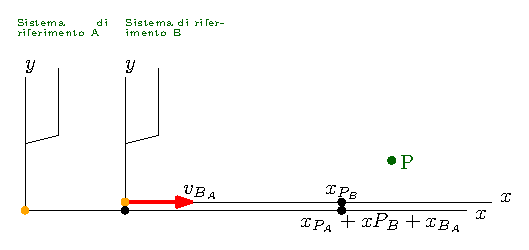
\includegraphics{img/motorelun.eps}
  \caption{Moto relativo Uniforme}
  \label{fig:motorel}
\end{figure}
\begin{eqnarray}
  \label{eq:morelauni}
  x_{BA}=\text{coord }B\text{ nel sistema di } A\\
  x_{PB}=\text{coord }P\text{ nel sistema di } B\\
  x_{PA}=x_{PB}+x_{BA} \text{coord }P\text{ nel sistema di } A
\end{eqnarray}

\section{Dinamica}
\label{sec:din}

\subsection{$2^a$ legge della dinamica}
\label{sec:2leggedin}
\begin{equation}
  \label{eq:2leggedin}
  \vec{F}=m\vec{a}
\end{equation}

\subsection{$3^a$ legge della dinamica}
\label{sec:3leggedin}
\begin{equation}
  \label{eq:3leggedin}
  F_{ab}=F_{ba}
\end{equation}

\subsection{Forza peso}
\label{sec:forzapeso}

\begin{equation}
  \label{eq:fp}
  P=m\cdot g
\end{equation}

\subsection{Forza di attrito}
\label{sec:forzad}

\begin{eqnarray}
  \label{eq:fds}
  F_{s}=\mu_sF_N\\
  F_k=\mu_kF_N
\end{eqnarray}

\section{Lavoro ed energia cinetica}
\label{sec:lavoroenecin}

\subsection{Energia cinetica}
\label{sec:enecin}

\begin{eqnarray}
  \label{eq:energiacinetica}
  K=\frac{1}{2}mv^2\\
  1J= 1kg \frac{m^2}{s^2}
\end{eqnarray}
\begin{teo}
  \begin{equation}
    \label{eq:teoen}
    \Delta{}K= K_j-K_i=L
  \end{equation}
  \begin{equation}
    \label{eq:lavoro}
    L=F*S
  \end{equation}
  \begin{itemize}
  \item \texttt{F} = forza;
  \item \texttt{S} = Spostamento.
  \end{itemize}
\end{teo}

\subsection{Energia elastica}
\label{sec:enelastica}

\begin{equation}
  \label{eq:enelast}
  U=\frac{1}{2}kS^2
\end{equation}

\subsection{Potenza}
\label{sec:potenza}

\begin{eqnarray*}
  \bar{P}=\frac{L}{\Delta{}t} \text{ Potenza media}\\
  P=\frac{dL}{dt} \text{ Potenza istantanea}
\end{eqnarray*}
\begin{center}
  1watt = 1J/s
\end{center}

\subsection{Energia potenziale gravitazionale}
\label{sec:enpotgrav}
\begin{equation}
  \label{eq:enpotgrav}
  U_g=m*g*h
\end{equation}

\subsection{Conservazione dell'energia meccanica}
\label{sec:condelmecc}

\begin{equation}
  \label{eq:emec}
  E_{mec}=K+U
\end{equation}
Conservazione dell'energia meccanica
\begin{equation}
  \label{eq:consenmec}
  K_2+U_2=K_1+U_1
\end{equation}

\subsection{Conservazione dell'energia}
\label{sec:consen}

\begin{equation}
  \label{eq:entot}
  L=\Delta{}E= \Delta{} E_{mecc} + \Delta{} E_{int} + \Delta{} E_{est}
\end{equation}

\section{Corpi rigidi e quantità di moto}
\label{sec:centrigequadimot}

\begin{equation}
  \label{eq:cdm}
  x_{cdm}=\frac{m_1 x_1+m_2x_2}{M}
\end{equation}

\subsection{Seconda legge di Newton}
\label{sec:seclegdiNew}
\begin{equation}
  \label{eq:seclegNew}
  \vec{F}=m*a
\end{equation}

\subsection{Quantità di moto o Momento lineare}
\label{sec:mv}

\begin{equation}
  \vec{P}=m\vec{v}
\end{equation}

\subsection{Urto e impulso}
\label{sec:urim}

\begin{equation}
  \label{eq:urtoeimp}
  \vec{F}=\frac{\Delta{}\vec{p}}{\Delta{}t}
\end{equation}

\subsection{Urti anelastici in una dimensione}
\label{sec:urtianelasticiinundim}

\begin{equation}
  \label{eq:urtianelundim}
  m_!\vec{v}_{1i}=\underbrace{\left(m_1+m_2\right)}_{\vec{v}_f=\frac{m_1}{m_1+m_2}\vec{v}_{1i}} v_f
\end{equation}

\subsection{Urti elastici in una dimensione}
\label{sec:urtelastinunadim}

\begin{eqnarray}
  \label{eq:urtelastinunadim}
  \begin{matrix}
    \vec{P}_f=\vec{P}_i; & K_f = K_i
  \end{matrix}\\
  \begin{cases}
    m_1\vec{v}_{1i}+m_2\vec{v}_{2i}=m_1\vec{v}_f+m_2\vec{v}_{2f}\\
    \frac{1}{2}m_1v_i^2+\frac{1}{2}m_2v_{2i}^2=\frac{1}{2}m_2v_{2f}^2
  \end{cases}
\end{eqnarray}

\subsection{Urti in due dimensioni}
\label{sec:urtiind2}

\begin{eqnarray}
  \label{eq:urtiind2}
  \vec{P}_{1i}+\vec{P}_{2i} = \vec{P}_{2f} + \vec{P}_{2f}\\
  K_{1i}+K_{2i} = K_{2f} + K_{2f}\\
  \begin{matrix}
    \text{comp }x & m_1\vec{v}_{1i}= m_1v_{1f}\cos{\Theta{}}+m_2v_{2f}\cos{\Theta{}}_2\\
    \text{comp }y & O =  -m_1v_{1f}\sin{\Theta{}}+m_2v_{2f}\sin{\Theta{}}_2
  \end{matrix}
\end{eqnarray}

\subsection{Sistemi a massa variabile}
\label{sec:sistemiamasvar}


\end{document}
